\begin{multicols}{2}
	\begin{test}[Newton's (second) law]{F = \frac{dp}{dt}}
		Defines both force and mass. Better known as $F = ma$, i.e. the net force on a body dictates exactly the rate of change of it's momentum.
	\end{test}
	
	\begin{test}[Momentum]{p = m\dot{x}}
		Total momentum in a system is conserved (as can be intuited assuming only elastic collisions, or derived via spatial symmetry and Noether's theorem)
	\end{test}
	\begin{test}[Work]{\displaystyle W = \int F ds}
		Taken here along a straight line path spanned by $x$, work is the line integral of Force by a line element of some path.
		\begin{equation*}
			W = \int F dx = \int \frac{dp}{dt} dx
		\end{equation*}
		However, $m \frac{dx}{dt} = p$ therefore $dx = \frac{p}{m} dt$ 
		\begin{equation*}
			W = \int \frac{p}{m} dp = \frac{p^2}{2m}
		\end{equation*}
	\end{test}
	\begin{test}[Kinetic Energy]{E_k = \frac{1}{2} m |\dot{q}|^2}
		Although the expression for the kinetic energy can be obtained via an integral, it - in order to fit what how we would expect a \textit{kinetic} energy to behave - must be some function of the magnitude of the velocity rather than favouring some direction (space is isotropic). Usually stated as $p^2 / 2m$ in Quantum Mechanics as the momentum operator is more fundamental (or solely valid).
		    
		Smacking chickens with hands at multiples of a large speed will reveal proportionality with mass and a quadratic relationship with speed.
	\end{test}
	\begin{test}[Potential]{F = -\frac{\partial V}{\partial q}}
		If a bit of (conservative) work $W$ is done on a system, the energy 
		
		\begin{equation*}
		    2 + 2 - 
		\end{equation*}
	\end{test}
\end{multicols}
\newpage
\section{Applications}
\subsection{Harmonic Oscillators}
%\begin{multicols}{2}
\begin{bigtest}[The Harmonic Oscillator]{\ddot{x} = -\omega^2_0 x}
	This equation (as can also be stated as Hooke's law $F= - kx$), dictates the motion of a harmonic oscillator. By substituting the Ansatz  $x = e^{kt}$, we obtain $k^2 = -w_0^2 \implies k = \pm iw_0$: From the linearity of the Differential Equation, a linear combination of these two solutions is also a solution and therefore we can write $x = Ae^{iw_0} + Be^{-iw_0}$
\end{bigtest}
\subsubsection{Damping an oscillator}
\begin{bigtest}[The Damped Harmonic Oscillator]{\ddot{x} + 2\gamma\dot{x} + \omega_0^2x = 0}
	By introducing a damping force $-bv$ we obtain
	\begin{equation*}
		F = -kx - b \dot{x}
	\end{equation*}
	This can be rearranged to obtain the form in blue, via introducing $\gamma = \frac{b}{2m}$ and $\omega_0 = \sqrt{k/m}$. Via the Ansatz $x = e^{gt}$, a quadratic equation and it's solutions are obtained:
	\begin{equation*}
		g = -\gamma \pm \sqrt{\gamma^2 - w_0^2}
	\end{equation*}
	                
	Upon inspection of the square root term, there are three cases of interest.
	                
	\begin{enumerate}
		\item Overdamping: $\gamma > \omega_0$. Obviously, we can see that $\gamma^2 - w_0^2 > 0$ which therefore means g has no imaginary component and therefore does not oscillate.
		      \begin{equation*}
		      	x = e^{-yt} (Ae^{t\sqrt{\gamma^2 - w_0^2}} + Be^{t\sqrt{\gamma^2 - w_0^2}})
		      \end{equation*}
		      Where $A, B$ are constants determined by the conditions imposed by a given system.
		\item Critical Damping: $\gamma = \omega_0$. 
		      \begin{equation*}
		      	g = - \gamma \pm  \cancel{ \sqrt{\gamma^2 - w_0^2}}
		      \end{equation*}
		      Therefore \textit{a} solution is $\ell = e^{-\gamma t}$. However, via hindsight we will investigate solutions of the form $x(t) = f(t)\ell(t)$.
		                          
		      Substituting our guess into our equation yields: 
		      \begin{align*}
		      	0 & = \ddot{x} + 2\gamma\dot{x} + \omega_0^2x                                                                    \\
		      	0 & = (\ddot{\ell}f + 2\dot{\ell}\dot{f} + \ell\ddot{f}) + 2\gamma(\dot{\ell}f + \ell\dot{f}) + \omega_0^2\ell f 
		      \end{align*}
		      Which can be rearranged to 
		      \begin{equation*}
		      	\ddot{f} \ell + \dot{f}(2\dot{\ell} + 2\gamma\ell) + f(\ddot{\ell} + 2\gamma\dot{\ell} + \omega_0^2\ell) = 0
		      \end{equation*}
		      The coefficient of $\dot{f}$ reduces to $\frac{d}{dt} e^{-\gamma t} = - \gamma e^{-\gamma t}$ i.e. $0$. The coefficient of $f$ is clearly zero as this is simply the statement (as we have already determined) $\ell$ solves the equation. This leaves us only with a condition on the derivatives of $f$: ${\ell > 0}_{\forall t}$ so $\ddot{f} = 0$
		      \begin{equation*}
		      	f = A + Bt
		      \end{equation*}
		      For this to be a distinct solution $b$ must be non-zero.
		      Therefore the solution is 
		      \begin{equation*}
		      	x(t) = (A + Bt)e^{-\gamma t}
		      \end{equation*}
		                          
		\item Underdamping: $\gamma < \omega_0$. In the underdamped case, $\gamma^2 - \omega_0^2 < 0$ and therefore g now has a non-zero imaginary part therefore the solution oscillates. 
		                          
		      \begin{equation*}
		      	g = -\gamma \pm \sqrt{\gamma^2 - w_0^2} = -\gamma \pm i\sqrt{w_0^2 - \gamma^2 }
		      \end{equation*}
		      Letting $\omega^{\star} = \sqrt{w_0^2 - \gamma^2} $Applying the usual linearity we get
		      \begin{align*}
		      	x & = Ae^{t(-\gamma + i\omega^{\star})} + Be^{t(-\gamma - i\omega^{\star})}        \\
		      	x & = e^{-\gamma t}[(A + B) \cos(t\omega^{\star}) + (A - B) \sin(t\omega^{\star})] 
		      \end{align*}
		      In order to obtain a real solution we dictate that $A + B$ and $A - B$ be real. Judicious application of trigonometric identities allow us to write the final solution as
		      \begin{equation*}
		      	x = Ce^{-\gamma t}\sin(\omega^{\star}t + \delta)
		      \end{equation*}
		      Which we can cleanly separate into a sinusoidal oscillation of diminishing (exponential) amplitude.
	\end{enumerate}
\end{bigtest}
\subsection{Driving damped oscillators and resonance}
\begin{bigtest}[Driving a damped Oscillator]{\ddot{z} + 2\gamma\dot{z} + \omega_0^2z = F(t)}
    We can know explore the properties of our oscillator when there are other forces involved, specifically those of pure time dependence - referred to as driving forces because of their Independence from the dynamical variables of a system.
\end{bigtest}

\begin{bigtest}[A periodic driving force]{F(t) = Fe^{i\theta t}}
    We are looking for a particular solution $z$ that yields $Fe^{i\theta t}$.
    
    It stands to reason that the resulting motion is of the same frequency as the driving force asymptotically, therefore our trial solution is $z = Ae^{i\theta t}$ where A is a complex number (to include a phase lag, i.e. the oscillator is damped so it will not follow instantly). 
    
    To start of on the right foot, $A = a e^{-i\delta}$ encodes the phase and amplitude of how our oscillator behaves rather than $F$.
    
    Direct substitution of $z$ into our equation, yields 
    \begin{align*}
        e^{i\theta t}(-A\theta^2 + 2iA\gamma\theta + \omega_0^2A) &= Fe^{i\theta t} \\
        -\theta^2 + 2i\gamma\theta + \omega_0^2 &= \frac{F}{A} = \frac{F}{a e^{-i\delta}} \\
         &= \frac{F}{a} e^{i\delta}
    \end{align*}
    By equating real and imaginary parts we obtain
    \begin{align*}
        \omega_0^2 - \theta^2 &= \frac{F}{a}\cos(\delta) \\
        2\gamma\theta &= \frac{F}{a}\sin(\delta)
    \end{align*}
    We obtain formulae for $\delta$ and $a$ by dividing and squaring respectively. 
    Figure \ref{fig:drivingAmplitude} is a plot of the former.
    \begin{gather*} 
        a = \frac{F}{\sqrt{(\omega_0^2 - \theta^2)^2 +  4\gamma^2\theta^2}} \\
        \tan(\delta) = \frac{2\gamma\theta }{\omega_0^2 - \theta^2}
    \end{gather*}
    \begin{figure}[ht]
        \centering
        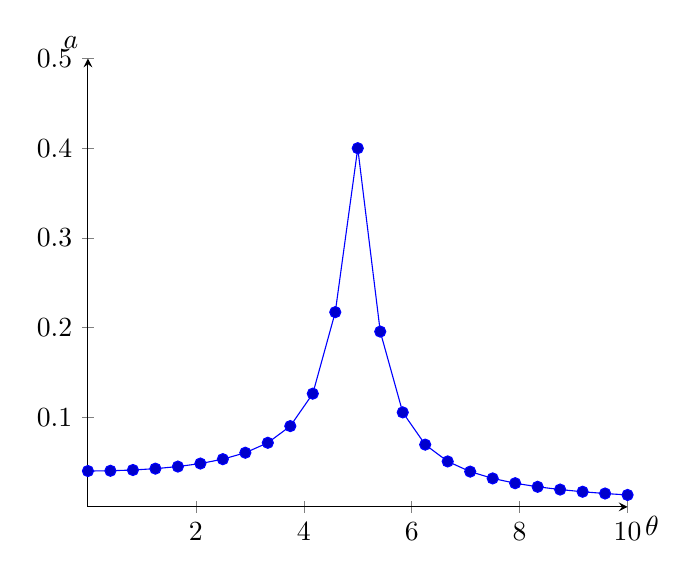
\begin{tikzpicture}
              \begin{axis}[
                      axis x line=center,
                      axis y line=center,
                      domain=0:10,
                      %xtick={0, 1,...,10},
                      ytick={0.1,0.2,...,1},
                      xlabel={$\; \theta$},
                      ylabel={$a$},
                      xlabel style={below right},
                      ylabel style={above left},
                      xmin=0,
                      xmax=10,
                      ymin=0,
                      ymax=0.5
                ]
                \addplot {1/(((25-x^2)^2 + 0.25*x^2))^0.5}; 
            \end{axis}
        \end{tikzpicture}
        \caption{Amplitude Against driving frequency}
        \label{fig:drivingAmplitude}
    \end{figure}
\end{bigtest}

\begin{bigtest}[Resonance]{a = \frac{F}{2 \gamma \sqrt{w_0^2 - \gamma^2}}}
    Taking our previously derived formula for the amplitude as a function of driving frequency, we can see a clear peak \textit{near} $\omega_0$. To investigate this we differentiate and set to zero our formula for the amplitude, yielding 
    
    \begin{align*}
        8\gamma^2\theta &= 4\theta(\omega_0^2 - \theta^2) \\
        \theta_r &= \sqrt{\omega_0^2 - 2\gamma^2}
    \end{align*}
    Where $\theta_r$ is the angular frequency at resonance. Substituting $\theta_r$ into our previously obtained expression for the amplitude yields the formula in blue. The phase lag can be evaluated accordingly.
    
    \paragraph{What do we have now}
    Having established the form and properties of this solution for a periodic driving force, we can either add it to the general solution to the non-driven case (to determine the behaviour at small times) or simply treat our particular solution as the asymptotic behaviour of the system over a long time period (i.e. a steady state solution).
\end{bigtest}

\subsection{Collisions}

